\section{Basic Assembly Test (BAT)}

\subsection{Purpose and Focus of the Test}
The purpose of the Basic Manipulation Test is to demonstrate basic assembly capabilities by the robots, like combining objects, by fitting or attaching them together.
\par
The focus is on the manipulation towards assembly, e.g.. force fitting or the preparation of objects to be attached by e.g.. external devices and machines.

\subsection{Scenario Environment}
The arena used for this test contains basically all elements as for the Basic Navigation Test. Additionally to environmental elements (walls, service areas, floor markers, etc.), different manipulatable objects will be placed on the service areas. 

\subsection{Manipulation Objects}
The manipulation objects in this test may include the objects specified in Table \ref{tab:manipulation_objects}. The set of objects is extended by:

\begin{table}[p]
\begin{tabular}{|c|c|c|c|}
\hline 
 & Symbolic Description & Weight (in g) & Details \\ 
\hline 
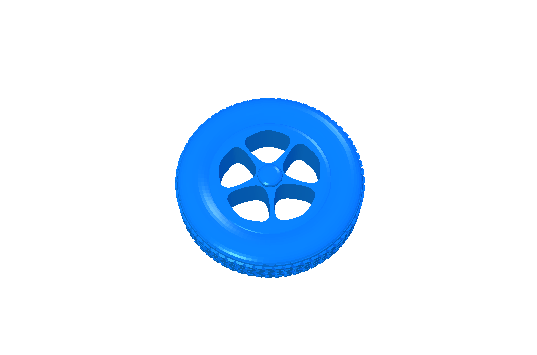
\includegraphics[width=3cm]{../images/BAT_Tire.png}  & T40 & approx. 50g & Height: 40mm \newline
 Width: 40mm \newline
 Length: approx. 10mm \\ 
\hline 

\label{tab:bat_objects}
\end{tabular} 
\caption{Examples of assembly objects}
\end{table}

\subsection{Task}
A single robot is used. The task consists of a sequence of assembly operations, with a small base movement in between. The objective is to collect a set of objects and perform an assembly option. This includes fitting a tire on an axle or assembling a bearing box. The task is finished once all objects are assembled or when the time foreseen for the run ends. 
\par
The task specification consists of: 
\begin{itemize}
	\item The specification of the initial place (e.g. D0, S5, U2)
	\item A location where to assemble
	\item The specification of a final place for the robot 
\end{itemize}

Two examples for a full task specification is as follows:
\begin{itemize}
	\item BAT\textless S2(T40,T40),A4(T40,T40),S7\textgreater  
\end{itemize}

\subsection{Rules}
The following rules have to be obeyed:

\begin{itemize}
\item The order in which the teams have to perform will be determined by a draw.
\item At the beginning of a team’s period, the team will get the task specification. 
\item The team must setup the robot in the designated start area.
\item A assembly object counts as successfully assembled when it is attached to the correct object or is in place for the external device to perform the assembly.
\end{itemize}


\subsection{Scoring}
Points are awarded as follows:

\begin{itemize}
\item 100 points are awarded for successfully assembling an assembly object that is part of the task specification..
\item -100 point for a wrong assembly
\end{itemize}

